% Created 2013-03-06 Wed 13:52
\documentclass[presentation]{beamer}
\usepackage[utf8]{inputenc}
\usepackage[T1]{fontenc}
\usepackage{fixltx2e}
\usepackage{graphicx}
\usepackage{longtable}
\usepackage{float}
\usepackage{wrapfig}
\usepackage{soul}
\usepackage{textcomp}
\usepackage{marvosym}
\usepackage[integrals]{wasysym}
\usepackage{latexsym}
\usepackage{amssymb}
\usepackage{hyperref}
\tolerance=1000
\usepackage{minted}
\usepackage{amsmath}
\usepackage{tikz}
\usepgflibrary{shapes.geometric}
\usetikzlibrary{calc}
\usetikzlibrary{positioning}
\usetheme{default}
\author{Lawrence Mitchell}
\date{\today}
\title{Source control and development practices}
\hypersetup{
  pdfkeywords={},
  pdfsubject={},
  pdfcreator={Generated by Org mode 7.9.3e in Emacs 24.3.50.1.}}
\begin{document}

\maketitle
\begin{frame}{Outline}
\tableofcontents
\end{frame}


\section{Mechanics}
\label{sec-1}

\begin{frame}[label=sec-1-1]{Source control}
\begin{itemize}
\item Git, Mercurial
\item excellent single-person repositories
\begin{itemize}
\item in addition, lots of neat distributed stuff
\end{itemize}
\end{itemize}
\end{frame}
\begin{frame}[label=sec-1-2]{Why bother}
\begin{itemize}
\item You work with existing code that uses VC
\item You're doing performance improvements on someone else's code
\item You're writing a paper (with or without people)
\item You want to be able to tie data to a particular version
\item \ldots{}
\end{itemize}
\end{frame}
\begin{frame}[fragile,label=sec-1-3]{Branching is easy (and cheap)}
 \begin{itemize}
\item Branches are a pain (IMO) in CVS and svn
\item not so in modern systems
\end{itemize}
\begin{minted}[frame=single,xleftmargin=1em,xrightmargin=1em,fontfamily=fi4]{sh}
git clone foo
git checkout -b new-branch
# hack hack
git commit
git checkout master
git merge new-branch
\end{minted}
\end{frame}
\begin{frame}[label=sec-1-4]{Corollary}
\begin{itemize}
\item Do it!
\begin{itemize}
\item and learn how to use them
\end{itemize}
\item e.g. Optimising code:
\begin{itemize}
\item a branch per optimisation
\item benchmark each one separately
\item benchmark combinations by merging branches
\end{itemize}

\item Implementing new features
\begin{itemize}
\item while maintaining "stable" trunk state
\end{itemize}
\end{itemize}
\end{frame}
\begin{frame}[fragile,label=sec-1-5]{Maintaining a "stable" trunk}
 \begin{itemize}
\item Develop on feature branches!
\item All trunk commits are merges
\begin{itemize}
\item tested!
\end{itemize}
\end{itemize}

\begin{minted}[frame=single,xleftmargin=1em,xrightmargin=1em,fontfamily=fi4]{sh}
git checkout -b feature/new-stuff
# hack hack hack
git commit # as and when
# test result of merge
git checkout -b tmp master
git merge feature/new-stuff
make test
git checkout master
git merge feature/new-stuff
# a tested complete feature
git push
\end{minted}
\begin{itemize}
\item Don't continually back-merge new changes from trunk
\begin{itemize}
\item unless necessary for your feature
\end{itemize}
\end{itemize}
\end{frame}
\begin{frame}[label=sec-1-6]{Pictures}
\begin{center}
\only<1>{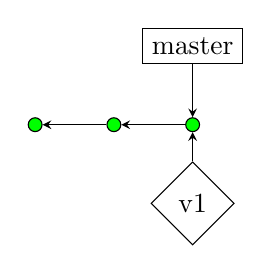
\begin{tikzpicture}

\tikzstyle{commit}=[draw, circle, inner sep=0pt,
                    minimum width=5pt]

\tikzstyle{master}=[fill=green]
\tikzstyle{featureB}=[fill=blue]
\tikzstyle{featureA}=[fill=orange]
\tikzstyle{branch}=[draw, rectangle]
\tikzstyle{tag}=[draw, diamond]
\tikzstyle{merge}=[diamond,inner sep=0pt, minimum size=5pt]
\node[commit, master] (A) {};
\node[commit, master] (B) [right of=A] {};
\node[commit, master] (C) [right of=B] {};

\draw[<-, >=stealth] (A) -- (B);
\draw[<-, >=stealth] (B) -- (C);


\node[branch] (master) [above of=C] {master};
\node[tag] (v1) [below of=C] {v1};
\draw[<-, >=stealth] (C) -- (master);
\draw[<-, >=stealth] (C) -- (v1);

\end{tikzpicture}
}
\only<2>{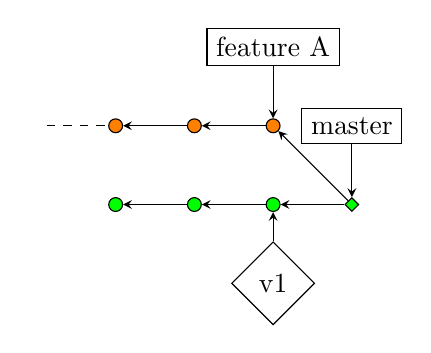
\begin{tikzpicture}

\tikzstyle{commit}=[draw, circle, inner sep=0pt,
                    minimum width=5pt]

\tikzstyle{master}=[fill=green]
\tikzstyle{featureB}=[fill=blue]
\tikzstyle{featureA}=[fill=orange]
\tikzstyle{branch}=[draw, rectangle]
\tikzstyle{tag}=[draw, diamond]
\tikzstyle{merge}=[diamond,inner sep=0pt, minimum size=5pt]
\node[commit, master] (A) {};
\node[commit, master] (B) [right of=A] {};
\node[commit, master] (C) [right of=B] {};

\draw[<-, >=stealth] (A) -- (B);
\draw[<-, >=stealth] (B) -- (C);


\node[commit,featureA] (C') [above of=C] {};
\node[commit,featureA] (B') [left of=C'] {};
\node[commit,featureA] (A') [left of=B'] {};
\node (Z) [left of=A'] {};
\draw[<-, >=stealth] (B') -- (C');
\draw[<-, >=stealth] (A') -- (B');
\draw[dashed] (Z) -- (A');
\node[commit,master,merge] (mergeA) [right of=C] {};
\draw[<-, >=stealth] (C') -- (mergeA);
\draw[<-, >=stealth] (C) -- (mergeA);

\node[branch] (master) [above of=mergeA] {master};
\node[branch] (featureA) [above of=C'] {feature A};

\node[tag] (v1) [below of=C] {v1};
\draw[<-, >=stealth] (mergeA) -- (master);
\draw[<-, >=stealth] (C') -- (featureA);
\draw[<-, >=stealth] (C) -- (v1);

\end{tikzpicture}
}
\only<3>{\input{03-06-EPCC-source-control.figures/branching-3.tikz}}
\only<4>{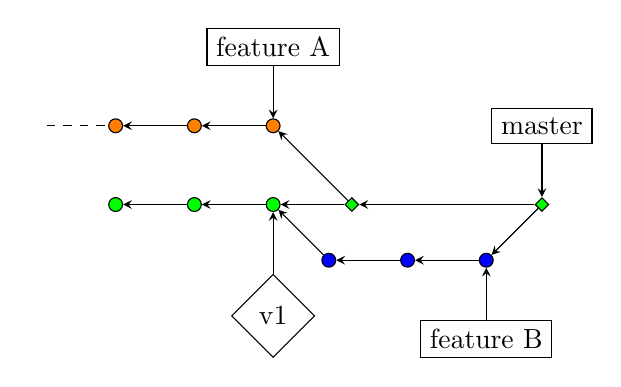
\begin{tikzpicture}

\tikzstyle{commit}=[draw, circle, inner sep=0pt,
                    minimum width=5pt]

\tikzstyle{master}=[fill=green]
\tikzstyle{featureB}=[fill=blue]
\tikzstyle{featureA}=[fill=orange]
\tikzstyle{branch}=[draw, rectangle]
\tikzstyle{tag}=[draw, diamond]
\tikzstyle{merge}=[diamond,inner sep=0pt, minimum size=5pt]
\node[commit, master] (A) {};
\node[commit, master] (B) [right of=A] {};
\node[commit, master] (C) [right of=B] {};

\draw[<-, >=stealth] (A) -- (B);
\draw[<-, >=stealth] (B) -- (C);


\node[commit, featureB] (C'') [below right of=C] {};
\node[commit, featureB] (D'') [right of=C''] {};
\node[commit, featureB] (E'') [right of=D''] {};

\draw[<-, >=stealth] (C) -- (C'');
\draw[<-, >=stealth] (C'') -- (D'');
\draw[<-, >=stealth] (D'') -- (E'');

\node[commit,featureA] (C') [above of=C] {};
\node[commit,featureA] (B') [left of=C'] {};
\node[commit,featureA] (A') [left of=B'] {};
\node (Z) [left of=A'] {};
\draw[<-, >=stealth] (B') -- (C');
\draw[<-, >=stealth] (A') -- (B');
\draw[dashed] (Z) -- (A');
\node[commit,master,merge] (mergeA) [right of=C] {};
\draw[<-, >=stealth] (C') -- (mergeA);
\draw[<-, >=stealth] (C) -- (mergeA);

\node[branch] (featureB) [below of=E''] {feature B};
\node[branch] (featureA) [above of=C'] {feature A};

\node[tag] (v1) [below left of=C''] {v1};
\draw[<-, >=stealth] (C') -- (featureA);
\draw[<-, >=stealth] (E'') -- (featureB);
\draw[<-, >=stealth] (C) -- (v1);

\node[commit,master,merge] (mergeB) [above right of=E''] {};
\draw[<-, >=stealth] (E'') -- (mergeB);
\draw[<-, >=stealth] (mergeA) -- (mergeB);
\node[branch] (master) [above of=mergeB] {master};
\draw[<-, >=stealth] (mergeB) -- (master);

\end{tikzpicture}
}
\end{center}
\end{frame}

\begin{frame}[fragile,label=sec-1-7]{Finding and fixing errors}
 \begin{itemize}
\item Bisection
\begin{itemize}
\item find error in $N$ commits in $\log{N}$ steps
\end{itemize}
\end{itemize}
\begin{minted}[frame=single,xleftmargin=1em,xrightmargin=1em,fontfamily=fi4]{sh}
# trunk is broken, but v1.1 is good
git bisect start
git bisect bad
git bisect good v1.1
make test # see if it's good or bad
git bisect good/bad
# repeat
# or git bisect run make test
# (make test returns return 0 for good, 1 for bad)
\end{minted}
\end{frame}
\begin{frame}[fragile,label=sec-1-8]{Corollary}
 \begin{itemize}
\item \emph{All} commits should be buildable and testable
\begin{itemize}
\item at the very least all that are merged to trunk
\end{itemize}
\end{itemize}
\begin{minted}[frame=single,xleftmargin=1em,xrightmargin=1em,fontfamily=fi4]{sh}
# bad
# hack hack hack (feature/foo)
git commit -m "part working"
# hack hack hack
git commit -m "now builds"
git checkout master
git merge feature/foo
\end{minted}
\begin{itemize}
\item now automated bisection won't work as well
\end{itemize}
\end{frame}
\begin{frame}[fragile,label=sec-1-9]{But we don't write perfect code first time}
 \begin{itemize}
\item Fix up mistakes after the fact
\end{itemize}
\begin{minted}[frame=single,xleftmargin=1em,xrightmargin=1em,fontfamily=fi4]{sh}
# hack hack
git commit -m "sort of working"
# hack hack
git commit -m "fixed now"
# hack hack
git commit -m "oh no, here's another corner case"
git rebase -i HEAD~4
\end{minted}
\end{frame}
\begin{frame}[fragile,label=sec-1-10]{Code archaeology}
 \begin{itemize}
\item Why does this line of code do X?
\begin{itemize}
\item git blame (\texttt{C-x v g} in Emacs)
\item other editors are available
\end{itemize}
\end{itemize}
\end{frame}
\begin{frame}[label=sec-1-11]{Corollary I}
\begin{itemize}
\item Write good commit messages
\item This is a bit of an art
\end{itemize}
\end{frame}

\begin{frame}[fragile,label=sec-1-12]{Example}
 \begin{itemize}
\item To follow along at home
\end{itemize}
\begin{minted}[frame=single,xleftmargin=1em,xrightmargin=1em,fontfamily=fi4]{sh}
git clone git://git.kernel.org/pub/scm/git/git.git
git show 75f7b5
\end{minted}
\begin{minted}[frame=single,xleftmargin=1em,xrightmargin=1em,fontfamily=fi4]{diff}
diff --git a/perl/Git.pm b/perl/Git.pm
-use Time::Local qw(timelocal);
+use Time::Local qw(timegm);
-       my $gm = timelocal(gmtime($t));
-       my $sign = qw( + + - )[ $t <=> $gm ];
+       my $gm = timegm(localtime($t));
+       my $sign = qw( + + - )[ $gm <=> $t ];
\end{minted}
\end{frame}
\begin{frame}[fragile,label=sec-1-13]{Corresponding commit message}
 \begin{verbatim}
perl/Git.pm: fix get_tz_offset to properly handle
             DST boundary cases

When passed a local time that was on the boundary
of a DST change, get_tz_offset returned a GMT
offset that was incorrect (off by one hour).  This
is because the time was converted to GMT and then
back to a time stamp via timelocal() which cannot
disambiguate boundary cases as noted in its
documentation.
\end{verbatim}
\end{frame}
\begin{frame}[fragile,label=sec-1-14]{\ldots{} continued}
 \begin{verbatim}
Modify this algorithm, using an approach suggested
in

  http://article.gmane.org/gmane.comp.
  version-control.git/213871

to first convert the timestamp in question to two
broken down forms with localtime() and gmtime(),
and then compute what timestamps these two broken
down forms would represent in GMT (i.e. a timezone
that does not have DST issues) by applying
timegm() on them.  The difference between the
resulting timestamps is the timezone offset.

This avoids the ambigious conversion and allows a
correct time to be returned on every occassion.
\end{verbatim}
\end{frame}
\begin{frame}[label=sec-1-15]{Corollary II}
\begin{itemize}
\item Don't commit logically unrelated changes together
\begin{itemize}
\item not even things like typo fixes or rewrapping lines
\end{itemize}
\end{itemize}
\end{frame}
\begin{frame}[fragile,label=sec-1-16]{Adding things to a commit}
 \begin{itemize}
\item In git, stage changes in a commit
\begin{itemize}
\item then commit
\end{itemize}
\end{itemize}

\begin{minted}[frame=single,xleftmargin=1em,xrightmargin=1em,fontfamily=fi4]{sh}
# hack hack hack (two unrelated features)
# but maybe in the same file
git add -i
# select the changes corresponding to feature-A
# on patch-hunk level
git commit
git add -i
# select the other changes
git commit
\end{minted}
\end{frame}
\section{Collaboration}
\label{sec-2}

\begin{frame}[label=sec-2-1]{Do code review}
\begin{itemize}
\item Maybe you've reinvented a wheel
\item Maybe there's a better way to do X
\end{itemize}
\end{frame}
\begin{frame}[fragile,label=sec-2-2]{Writing a reviewable feature}
 \begin{itemize}
\item Order commits logically
\begin{itemize}
\item introduce a failing test demonstrating bug
\item fix bug
\item show how test passes
\end{itemize}
\item make each commit reviewable separately (in order)
\begin{itemize}
\item \texttt{git rebase} is your friend
\end{itemize}
\end{itemize}
\end{frame}
\begin{frame}[label=sec-2-3]{Corollary}
\begin{itemize}
\item Try to keep features "small"
\begin{itemize}
\item implement one thing at a time
\item merge features to master as you go
\end{itemize}
\end{itemize}
\end{frame}
\begin{frame}[fragile,label=sec-2-4]{Addressing comments}
 \begin{itemize}
\item Don't take criticism/nitpicking personally
\begin{itemize}
\item discuss things you disagree with though!
\end{itemize}
\item Don't add fixups on top
\item Rework the existing patches
\end{itemize}
\begin{minted}[frame=single,xleftmargin=1em,xrightmargin=1em,fontfamily=fi4]{sh}
# address issue A
git commit -m "fixA"
# fix issue B
git commit -m "fixB"
git rebase -i ...
# squash fixA/fixB into appropriate commit
\end{minted}
\end{frame}
\section{Testing and verification}
\label{sec-3}

\begin{frame}[label=sec-3-1]{Testing I}
\begin{itemize}
\item How long does it take a developer to kick off a test of their code
branch?
\begin{itemize}
\item 30 minutes?
\item 5 minutes?
\item 1 minute?
\item 1 second?
\end{itemize}
\end{itemize}
\end{frame}
\begin{frame}[label=sec-3-2]{Testing II}
\begin{itemize}
\item Make it easy to \emph{write} tests
\begin{itemize}
\item commit to a standard test framework if possible
\end{itemize}
\item Encourage developers to write tests
\begin{itemize}
\item Don't let new features in without tests!
\end{itemize}
\end{itemize}
\end{frame}
\begin{frame}[label=sec-3-3]{Continuous integration servers}
\begin{itemize}
\item For example:
\begin{itemize}
\item Travis
\item Jenkins/Hudson
\item Buildbot
\end{itemize}
\item feature branches
\begin{itemize}
\item push a button to trigger tests on a branch
\item or auto-test on push if tests don't take hours
\item or run nightly tests on all branches
\end{itemize}
\item trunk
\begin{itemize}
\item any commit kicks off tests
\item mail developers when things break
\end{itemize}
\end{itemize}
\end{frame}
\begin{frame}[label=sec-3-4]{Continuous integration and code review}
\begin{itemize}
\item Code review platforms integrate with CI servers
\begin{itemize}
\item propose a merge
\item CI server does build and test of merged feature
\item flag failures in review system
\end{itemize}
\end{itemize}
\end{frame}
\section{Putting things together}
\label{sec-4}

\begin{frame}[label=sec-4-1]{Source control hosting}
\begin{itemize}
\item Github
\begin{itemize}
\item free for OS repos
\item pay for private
\item pay for self-hosted
\end{itemize}
\item Bitbucket
\begin{itemize}
\item free for OS repos
\item free private for academic users (us)
\end{itemize}
\item Gitorious
\begin{itemize}
\item similar
\end{itemize}
\end{itemize}
\end{frame}
\begin{frame}[label=sec-4-2]{Issues with third-party sites}
\begin{itemize}
\item URI stability
\item What happens if they disappear?
\begin{itemize}
\item you can get the repository data out
\item what about the issue trackers?
\end{itemize}
\item I don't have any good answers
\end{itemize}
\end{frame}
\begin{frame}[fragile,label=sec-4-3]{Code review options}
 \begin{itemize}
\item Github, Bitbucket
\begin{itemize}
\item pull requests + inline review
\end{itemize}
\item Gerrit
\begin{itemize}
\item self hosting option
\end{itemize}
\item Git at least designed for email-based workflow
\end{itemize}
\begin{minted}[frame=single,xleftmargin=1em,xrightmargin=1em,fontfamily=fi4]{sh}
# send changes to people
git send-email
# apply changes
git am mailbox
\end{minted}
\end{frame}
\begin{frame}[label=sec-4-4]{CI}
\begin{itemize}
\item Generally self-hosting
\begin{itemize}
\item But see Travis
\end{itemize}
\item Integrate with most major hosting sites
\end{itemize}
\end{frame}
\begin{frame}[label=sec-4-5]{That's all}
\begin{itemize}
\item Any questions?
\end{itemize}
\end{frame}
% Generated by Org mode 7.9.3e in Emacs 24.3.50.1.
\end{document}
